\subsection{ParallelMesh}

%%%%%%%%%%%%%%%%%%%%%%%%%%%%%%%%%%%%%%%%%%%%%%%%%%%%%%%%%%%%%%%%%%%%%
\royslide{Mesh Classes}{

\begin{columns}
\begin{column}{.5\textwidth}
  \begin{center}
    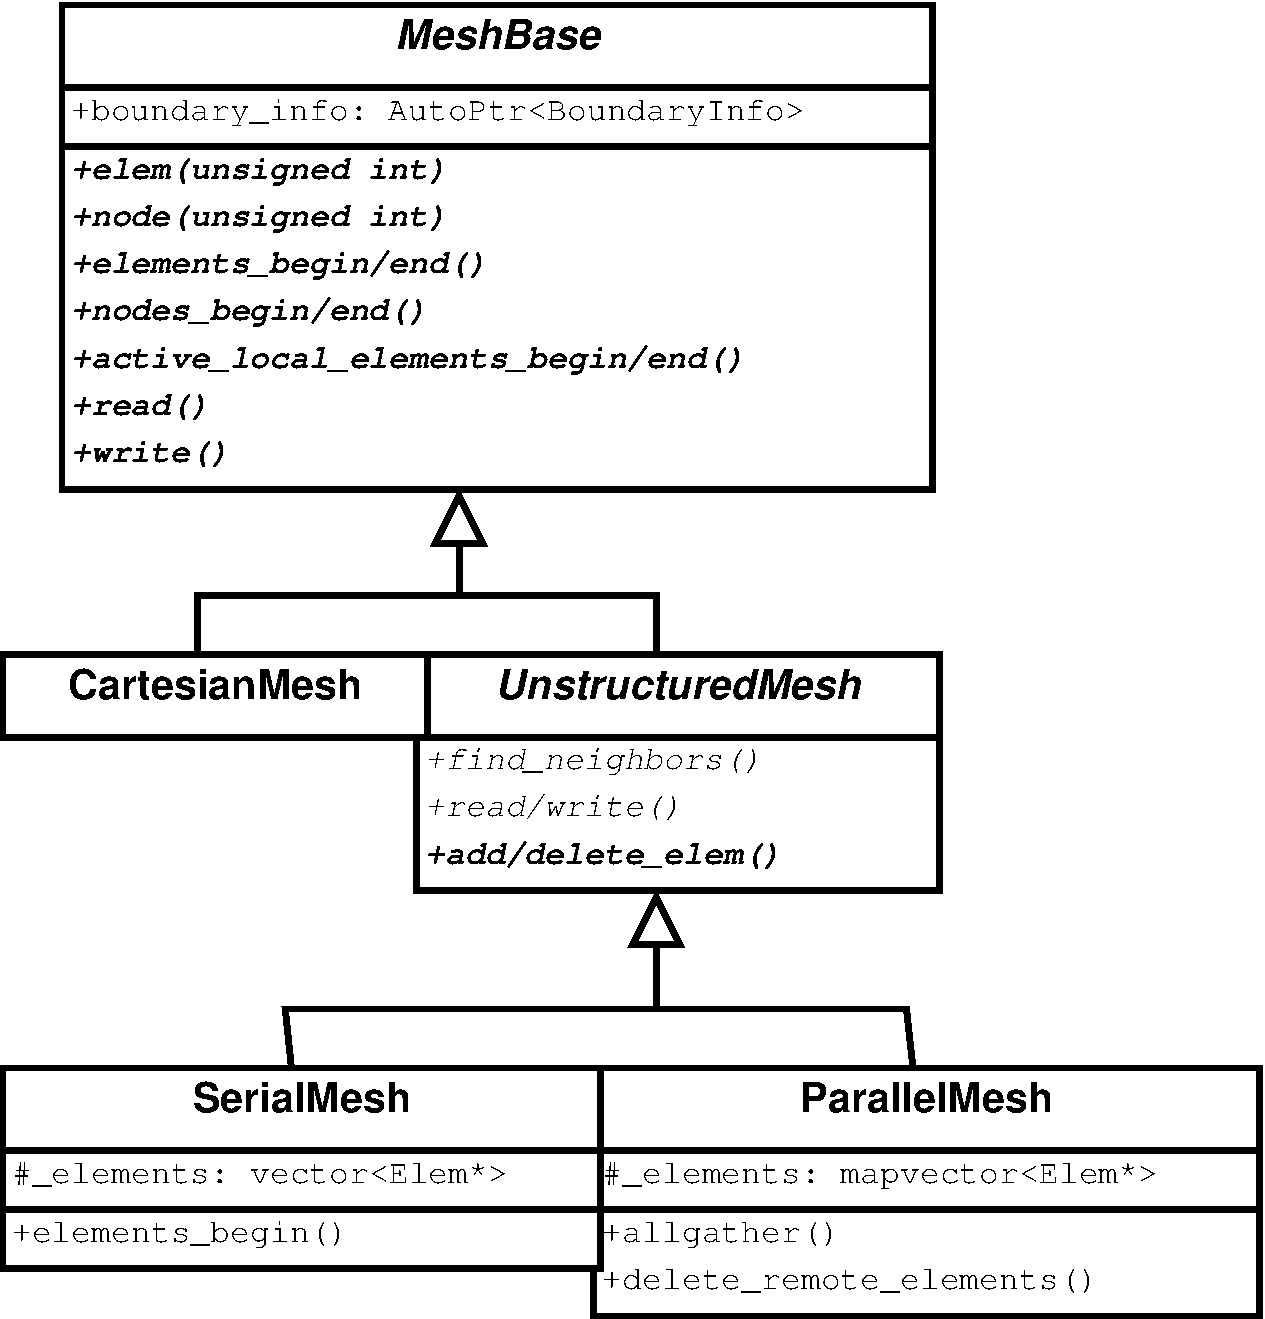
\includegraphics[width=.9\textwidth]{parallelism/MeshUML}
  \end{center}
\end{column}
\begin{column}{.5\textwidth}
  \royitemizebegin{}
    \item Abstract iterator interface hides mesh type from most applications
    \item UnstructuredMesh "branch" for most library code
    \item ParallelMesh implements data storage, synchronization
  \royitemizeend
\end{column}
\end{columns}
}



%%%%%%%%%%%%%%%%%%%%%%%%%%%%%%%%%%%%%%%%%%%%%%%%%%%%%%%%%%%%%%%%%%%%%
\royslide{SerialMesh Partitioning}{
\begin{columns}
\begin{column}{.5\textwidth}
  \royitemizebegin{}
    \item Each element, node is ``local'' to one processor
    \item Each processor has an identical Mesh copy
    \item Mesh stays in sync through redundant work
    \item FEM data synced on ``ghost'' elements only
  \royitemizeend
\end{column}
\begin{column}{.5\textwidth}
  \begin{center}
    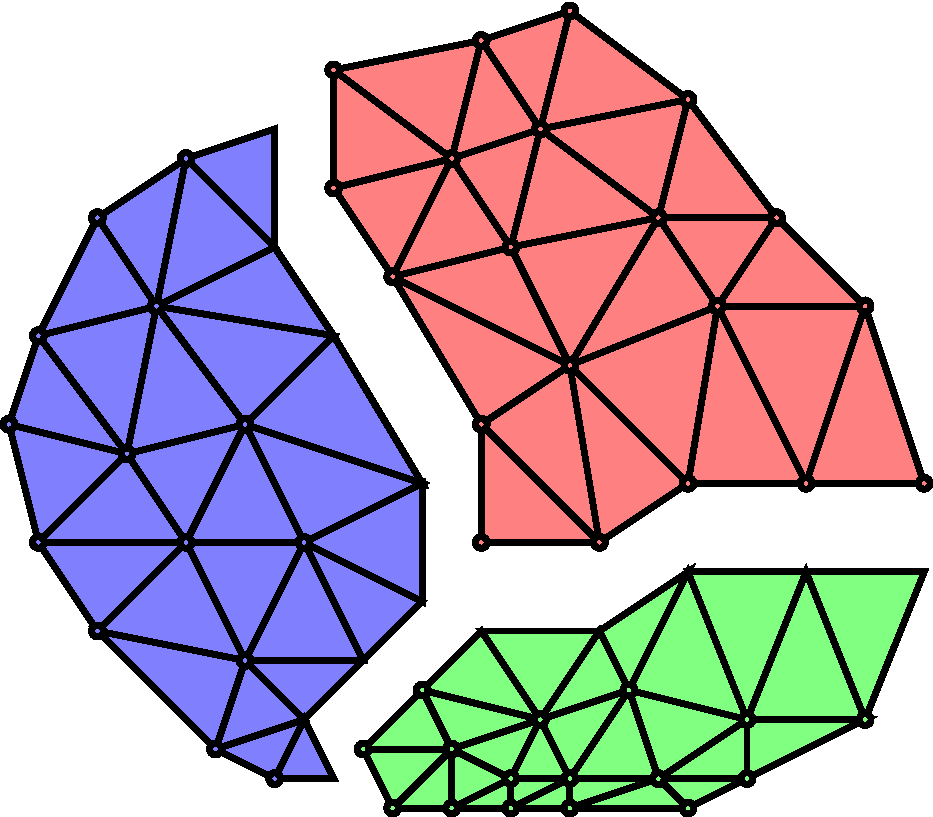
\includegraphics[width=.9\textwidth]{parallelism/SerialMesh}
  \end{center}
\end{column}
\end{columns}
}


%%%%%%%%%%%%%%%%%%%%%%%%%%%%%%%%%%%%%%%%%%%%%%%%%%%%%%%%%%%%%%%%%%%%%
\royslide{ParallelMesh Partitioning}{
\begin{columns}
\begin{column}{.5\textwidth}
  \royitemizebegin{}
    \item Processors store only local and ghost objects
    \item Each processor has a small Mesh subset
    \item Mesh stays in sync through MPI communication
  \royitemizeend
\end{column}
\begin{column}{.5\textwidth}
  \begin{center}
    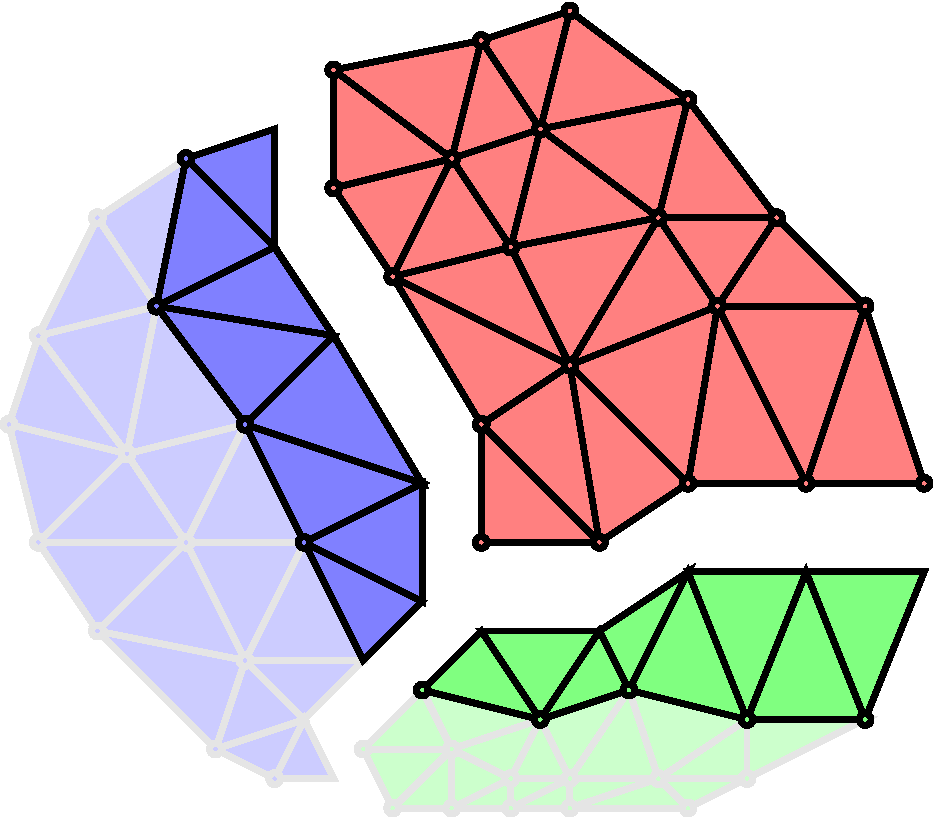
\includegraphics[width=.9\textwidth]{parallelism/ParallelMesh1}
  \end{center}
\end{column}
\end{columns}
}



%%%%%%%%%%%%%%%%%%%%%%%%%%%%%%%%%%%%%%%%%%%%%%%%%%%%%%%%%%%%%%%%%%%%%
\royslide{ParallelMesh Partitioning}{
\begin{columns}
\begin{column}{.5\textwidth}
  \royitemizebegin{Pros}
    \item Reduced memory use
    \item $O(N_E/N_P)$ CPU costs
  \royitemizeend
\end{column}
\begin{column}{.5\textwidth}
  \begin{center}
    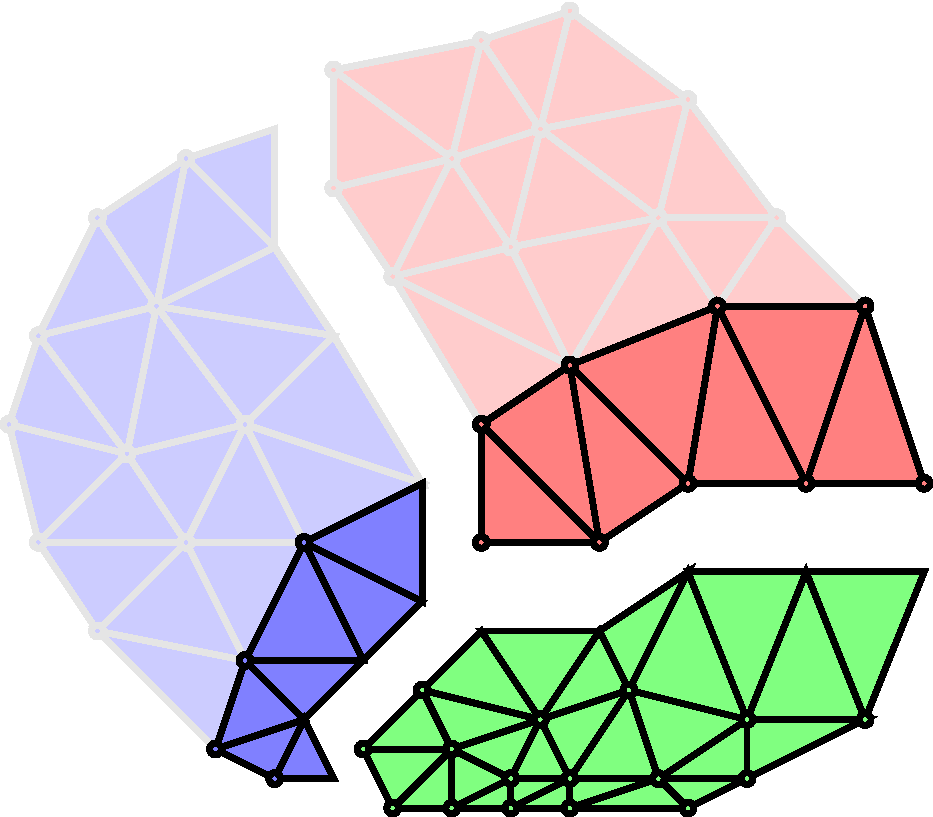
\includegraphics[width=.9\textwidth]{parallelism/ParallelMesh2}
  \end{center}
\end{column}
\end{columns}
}



%%%%%%%%%%%%%%%%%%%%%%%%%%%%%%%%%%%%%%%%%%%%%%%%%%%%%%%%%%%%%%%%%%%%%
\royslide{ParallelMesh Partitioning}{
\begin{columns}
\begin{column}{.5\textwidth}
  \royitemizebegin{Cons}
    \item Increased code complexity
    \item Increased synchronization ``bookkeeping''
    \item Greater debugging difficulty
  \royitemizeend
\end{column}
\begin{column}{.5\textwidth}
  \begin{center}
    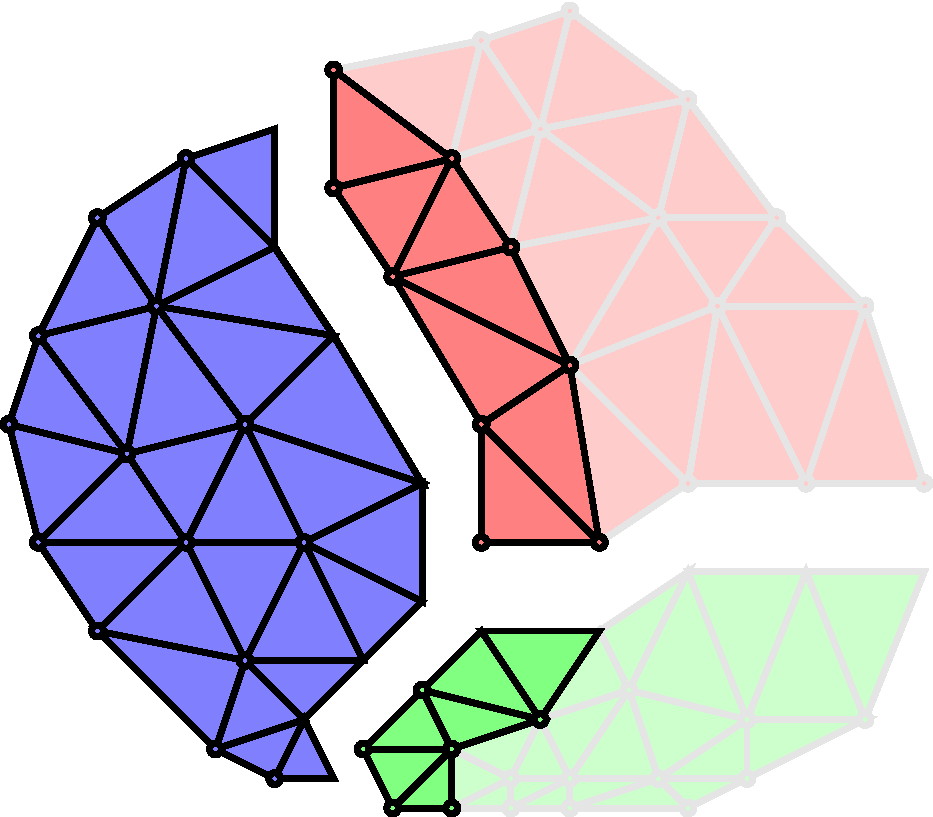
\includegraphics[width=.9\textwidth]{parallelism/ParallelMesh3}
  \end{center}
\end{column}
\end{columns}
}



%%%%%%%%%%%%%%%%%%%%%%%%%%%%%%%%%%%%%%%%%%%%%%%%%%%%%%%%%%%%%%%%%%%%%
\royslide{Gradual Parallelization}{
  \royitemizebegin{Starting from SerialMesh behavior}
    \item New internal data structure
    \item Methods to delete, reconstruct non-semilocal objects
    \item Parallelized DofMap methods
    \item Parallelized MeshRefinement methods
    \item Parallel Mesh I/O support
    \item Load balancing support
  \royitemizeend

  Also working on parallel support in Boundary, Function, Generation,
Modification, Generation, Tools classes
}


%===============================================================================
% NEW SLIDE
%===============================================================================
\begin{frame}
\frametitle{Distributed Mesh Refinement}

\begin{block}{Error Estimation}
\begin{itemize}
\item Local residual, jump error estimators\only<2->{: embarrassingly parallel}
\item Refinement-based estimators\only<2->{: use solver parallelism}
\item Adjoint-based estimators\only<2->{: use solver parallelism}
\item Recovery estimators\only<2->{: require partitioning-aware patch generation}
\end{itemize}
\end{block}

\visible<3->{
\begin{block}{Refinement Flagging}
\begin{itemize}
\item Flagging by error tolerance: $\eta_K^2 < \eta_{tol}^2/N_E$
\begin{itemize}
\item<4> Embarrassingly parallel
\end{itemize}
\item Flagging by error fraction: $\eta_K < r \max_K{\eta_K}$
\begin{itemize}
\item<4> One global Parallel::max to find maximum error
\end{itemize}
\item Flagging by element fraction or target $N_E$
\begin{itemize}
\item<4> Parallel::Sort to find percentile levels?
\item<4> Binary search in parallel?
\item<4> TBD
\end{itemize}
\end{itemize}
\end{block}
}

\end{frame}

%===============================================================================
% NEW SLIDE
%===============================================================================
\begin{frame}
\frametitle{Distributed Mesh Refinement}

\begin{columns}
\column{.6\textwidth}
\begin{block}{Elem, Node creation}
\begin{itemize}
\item<2-> Ids $\{i: i\;{\mathrm{mod}}\;(N_P+1) = p\}$ are owned by processor $p$
\end{itemize}
\end{block}

\visible<3->{
\begin{block}{Synchronization}
\begin{itemize}
\item Refinement Flags
\begin{itemize}
  \item<4-> Data requested by id
  \item<4-> Iteratively to enforce smoothing
\end{itemize}
\item New ghost child elements, nodes
\begin{itemize}
\item<4-> Id requested by data
\end{itemize}
\item Hanging node constraint equations
\begin{itemize}
\item<4-> Iteratively through subconstraints,
subconstraints-of-subconstraints...
\end{itemize}
\end{itemize}
\end{block}
}
\column{.4\textwidth}
\begin{center}
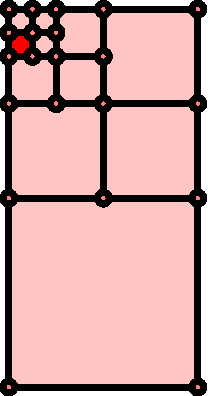
\includegraphics[width=.6\textwidth]{parallelism/LevelOneProblem}
\end{center}
\end{columns}

\end{frame}

%\section{Applications}

\subsection{Performance}

%===============================================================================
% NEW SLIDE
%===============================================================================
\begin{frame}
\frametitle{``Typical'' PDE example}

Transient Cahn-Hilliard, Bogner-Fox-Schmidt quads or hexes

  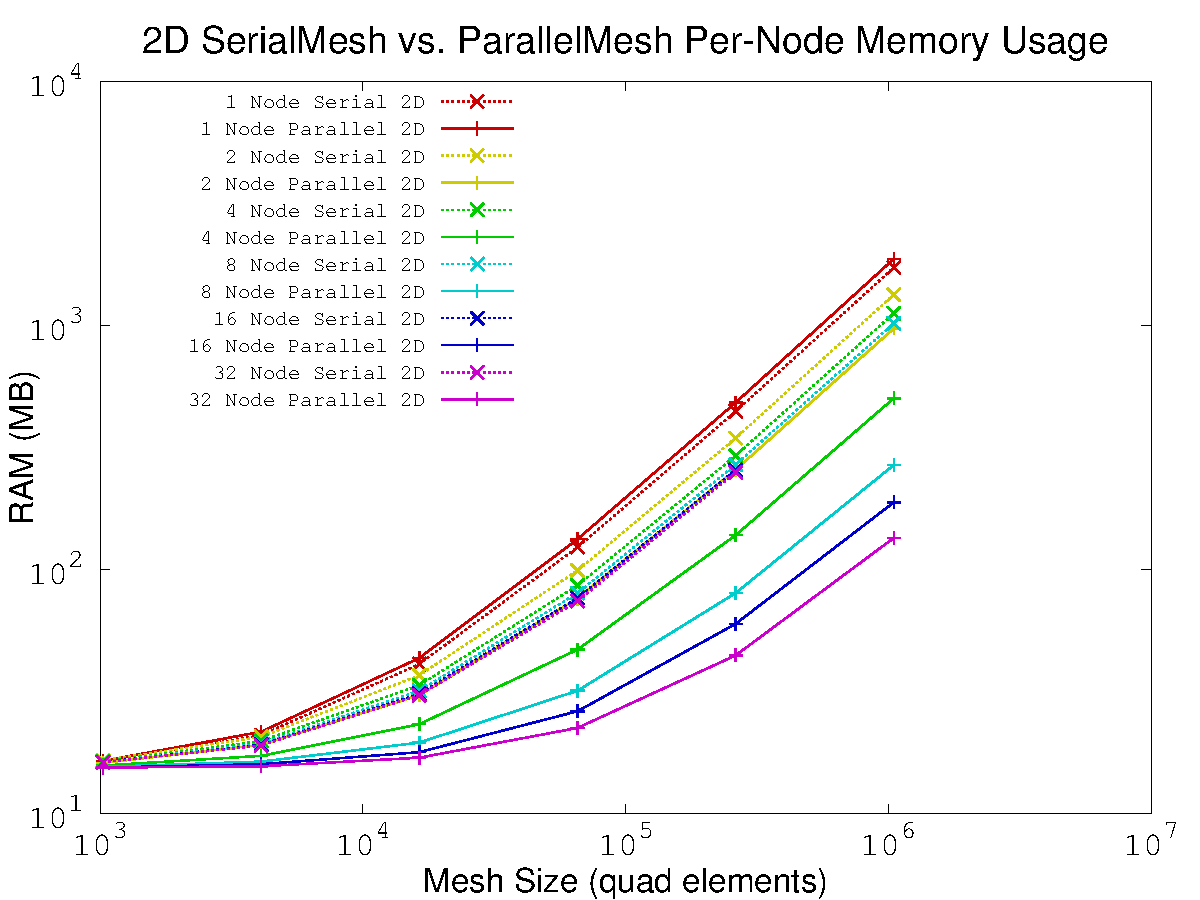
\includegraphics[width=.5\textwidth]{parallelism/parallelmesh_usage_2D}
  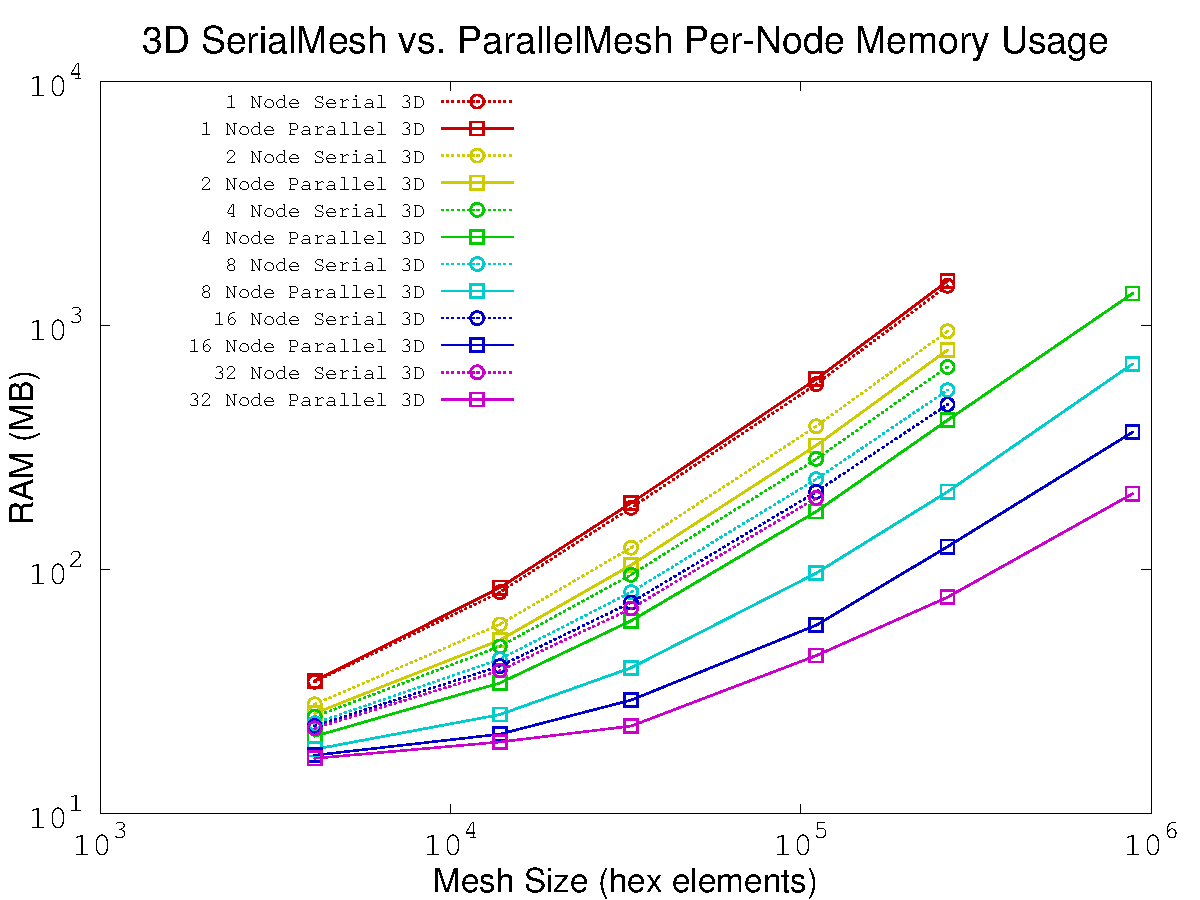
\includegraphics[width=.5\textwidth]{parallelism/parallelmesh_usage_3D}

\begin{block}{Results}
\begin{itemize}
\item Parallel codes using SerialMesh are unchanged for ParallelMesh
\item Overhead, distributed sparse matrix costs are unchanged
\item Serialized mesh, indexing once dominated RAM use
\end{itemize}
\end{block}
\end{frame}
